\documentclass{article}
\usepackage[cm]{fullpage} %very small margins (around 1.5cm)
\usepackage{url} %use \url{} in the document
\usepackage{graphicx} %images

\begin{document}

\title{Universal Game System specification}
\date{February 11, 2012}
\author{Bysiek Mateusz, Peryt Stanis�aw, Wi�niewski Adrian, Witan Maciej}
\maketitle

\tableofcontents

\section{Abstract}

\subsection{License}
Apache License 2.0

\subsection{Responsibilities}
This work is a result of collaboration of 4 people. To make things easier, 
we've made clear who's doing what, and included that information in this document.

\subsubsection{People}
\paragraph{Bysiek M.} E-mail: \url{bysiekm@student.mini.pw.edu.pl}
Class diagrams. Protocol definition. Input data definition.
\paragraph{Peryt S.} E-mail: \url{peryts@student.mini.pw.edu.pl}
Quality control, coordination of the work. This document.
\paragraph{Wisniewski A.} E-mail: \url{wisniewskia@student.mini.pw.edu.pl}
Use-case diagrams.
\paragraph{Witan M.} E-mail: \url{witanm@student.mini.pw.edu.pl}
Event flow diagrams. State diagrams. Activity diagrams.

\subsubsection{Material}
\begin{enumerate}
  \item Requirements Specification
  \begin{enumerate}
    \item System actors' use cases
    \begin{enumerate}
      \item person running a game server
      \item person running a game client
      \item a game client accessing and using game server
      \item game server communicating with game client
    \end{enumerate}
    All of the above: \url{wisniewskia}
  \end{enumerate}
  \item Complete Design Documentation (Game Server and Game)
  \begin{enumerate}
    \item Input data format specification: \url{bysiekm}
    \item Class diagrams describing structures, modules and architecture of the system: \url{bysiekm}
    \item Event flow diagrams describing interaction between game server and game applications: \url{witanm}
    \item State diagrams describing states of components of Game server and components of game applications: \url{witanm}
    \item Important activity diagrams describing overall activities of the server and clients: \url{witanm}
    \item Communication protocol design (if possible a set of XML tags): \url{bysiekm}
    \item Additional relevant comments: \url{peryts}
    \item Special system states description (initialization, shut down, failures): \url{peryts}
  \end{enumerate}
  \item Vocabulary (if needed): \url{peryts}
\end{enumerate}

\subsection{Github repo}
This document (written in LaTeX) and all diagrams (created in Visio) are available online 
in a open Github repository: \url{https://github.com/mbdevpl/UniversalGameSystem}

\section{Use-cases}
\subsection{Person running a game server}
\subsection{Person running a game client}

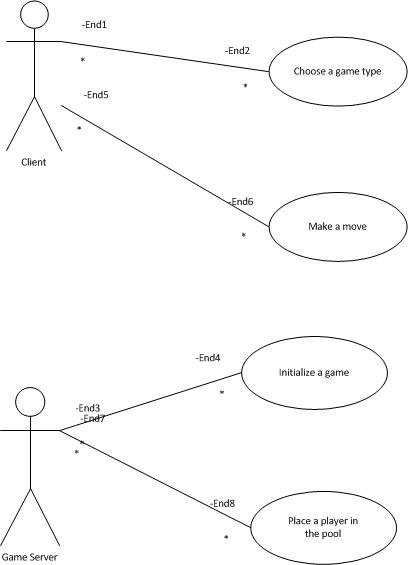
\includegraphics[scale=0.95]{UGS_usecases_client.jpg}

\subsection{A game client accessing and using game server}
\subsection{Game server communicating with game client}

\section{Input data format}

\section{Class diagrams}

\section{Event flow diagrams}
Interaction between game server and game applications.

\section{State diagrams}

\section{Activity diagrams}

\section{Communication protocol}

\section{Additional comments}

\section{Vocabulary}

\end{document}
